\subsection{Discrete Wavelet Transform}
% 
Conventionally, discrete wavelet transform attempts to decompose an image into two sub-regions: the upper-left stores the low frequency coefficients and the rest stores the high coefficients.
The main bottlenecks of this scheme are memory-bound issues when we have to either access non-contiguous memory or use image transposition. 
Although, the sliding window method can help us to quickly process the image without transposition, we still need to rearrange the coefficients after each filtering step. 
Using the mixed-band algorithm, we can achieve the higher performance of DWT by shuffling the wavelet spectrum and improve the contiguous memory access. 
It also fits elegantly to the GPU programming model. 

\begin{figure}[t]
	\centering  
	%%%%%%%%%%%%%%%%%%%%%%%%%%%%%%%%%%%%%%%%%%%%%%%%%%%%%%%%%%%%%%%%%%%%%%%
	\subfloat[]
    {  
  		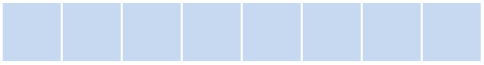
\includegraphics[width=0.3\linewidth]{fig/traditional1d0.png}
	}	\\
    \subfloat[]
    {
		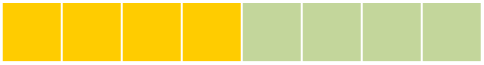
\includegraphics[width=0.3\linewidth]{fig/traditional1d1.png}
    }	
	\subfloat[]
    {  
  		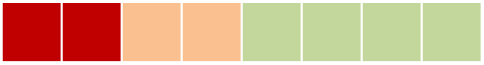
\includegraphics[width=0.3\linewidth]{fig/traditional1d2.png}
	}	
		\subfloat[]
    {  
  		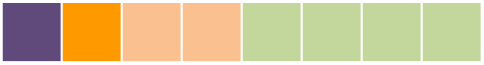
\includegraphics[width=0.3\linewidth]{fig/traditional1d3.png}
	}	\\
	\subfloat[]
    {
		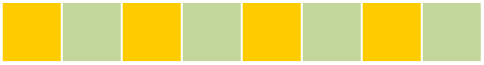
\includegraphics[width=0.3\linewidth]{fig/mixedband1d1.png}
    }	
	\subfloat[]
    {  
  		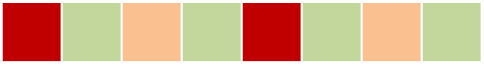
\includegraphics[width=0.3\linewidth]{fig/mixedband1d2.png}
	}	
		\subfloat[]
    {  
  		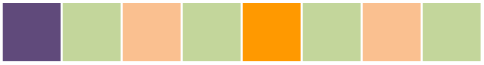
\includegraphics[width=0.3\linewidth]{fig/mixedband1d3.png}
	}	\\
	%%%%%%%%%%%%%%%%%%%%%%%%%%%%%%%%%%%%%%%%%%%%%%%%%%%%%%%%%%%%%%%%%%%%%%%
	\subfloat[]
	{  
		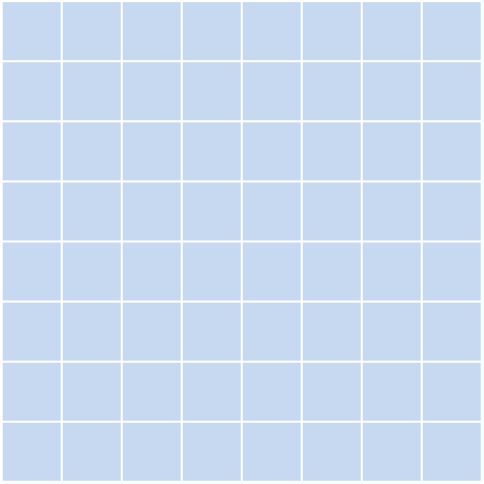
\includegraphics[width=0.3\linewidth]{fig/traditional2d0.png}
	}	\\
	\subfloat[]
	{
		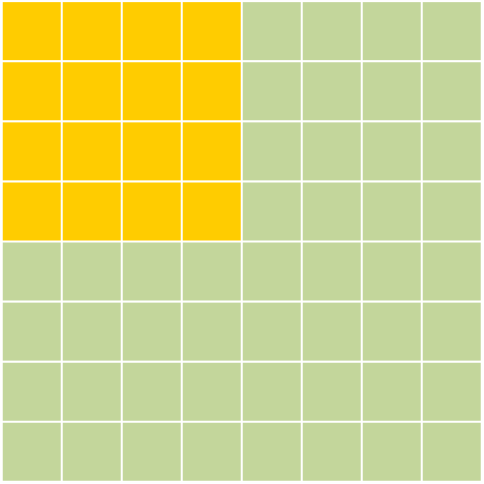
\includegraphics[width=0.3\linewidth]{fig/traditional2d1.png}
	}	
	\subfloat[]
	{  
		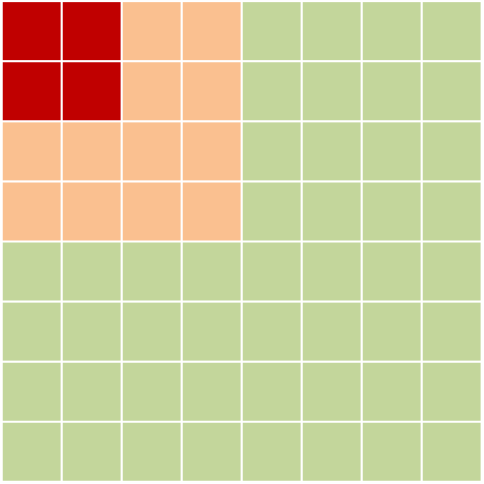
\includegraphics[width=0.3\linewidth]{fig/traditional2d2.png}
	}	
		\subfloat[]
	{  
		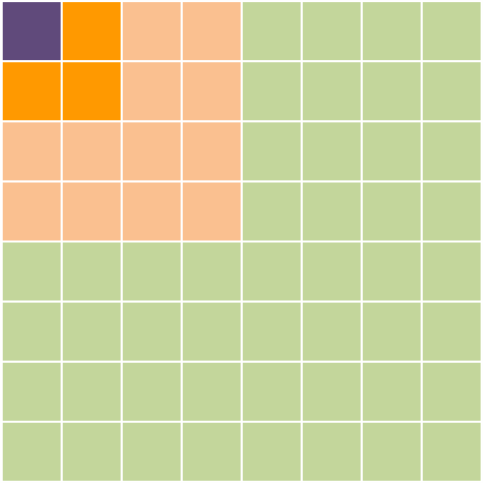
\includegraphics[width=0.3\linewidth]{fig/traditional2d3.png}
	}	\\
	\subfloat[]
	{
		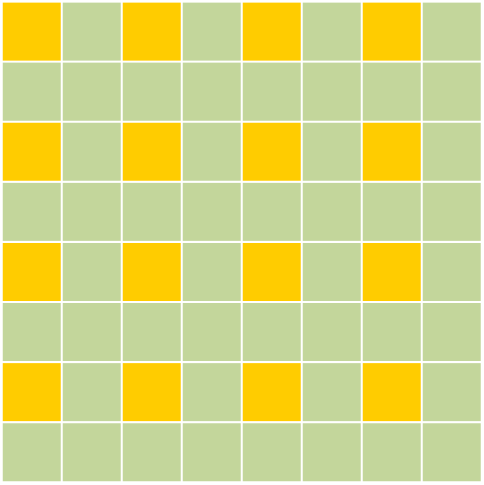
\includegraphics[width=0.3\linewidth]{fig/mixedband2d1.png}
	}	
	\subfloat[]
	{  
		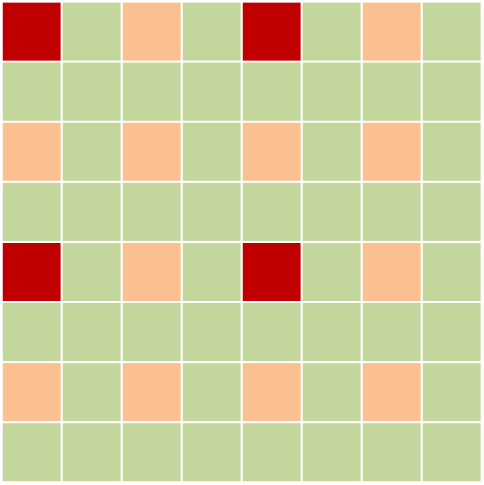
\includegraphics[width=0.3\linewidth]{fig/mixedband2d2.png}
	}	
		\subfloat[]
	{  
		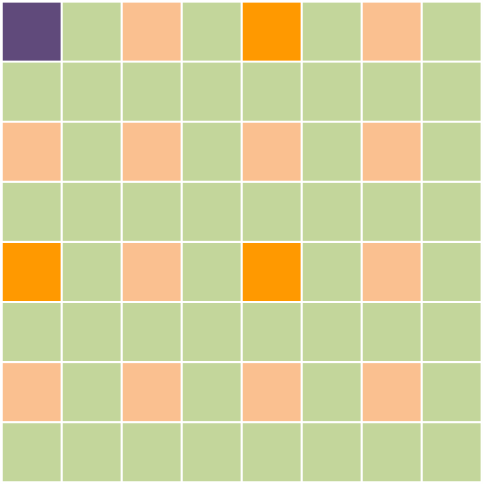
\includegraphics[width=0.3\linewidth]{fig/mixedband2d3.png}
	}	\\
	%%%%%%%%%%%%%%%%%%%%%%%%%%%%%%%%%%%%%%%%%%%%%%%%%%%%%%%%%%%%%%%%%%%%%%%
	\subfloat[]
	{  
		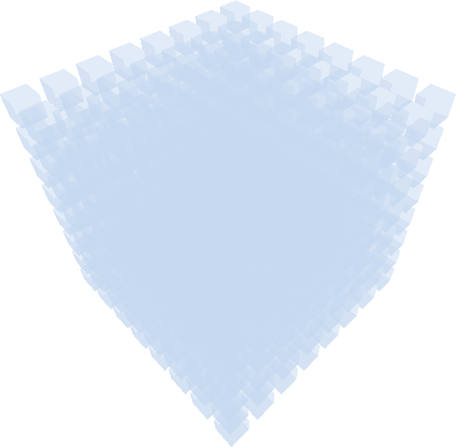
\includegraphics[width=0.3\linewidth]{fig/traditional3d0.png}
	}	\\
	\subfloat[]
	{
		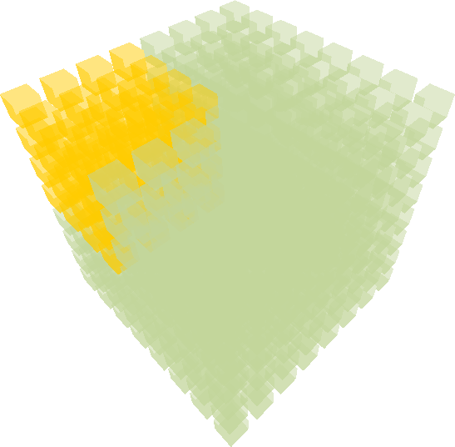
\includegraphics[width=0.3\linewidth]{fig/traditional3d1.png}
	}	
	\subfloat[]
	{  
		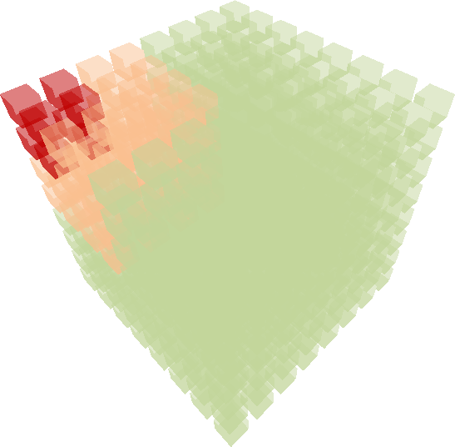
\includegraphics[width=0.3\linewidth]{fig/traditional3d2.png}
	}	
		\subfloat[]
	{  
		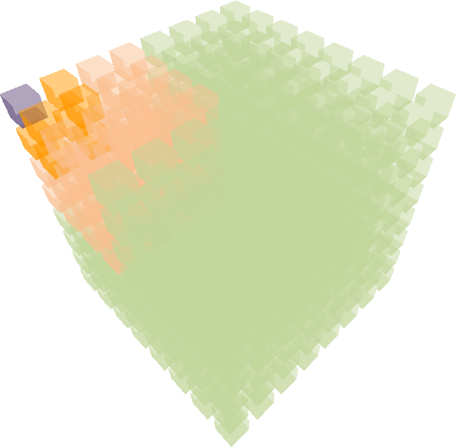
\includegraphics[width=0.3\linewidth]{fig/traditional3d3.png}
	}	\\
	\subfloat[]
	{
		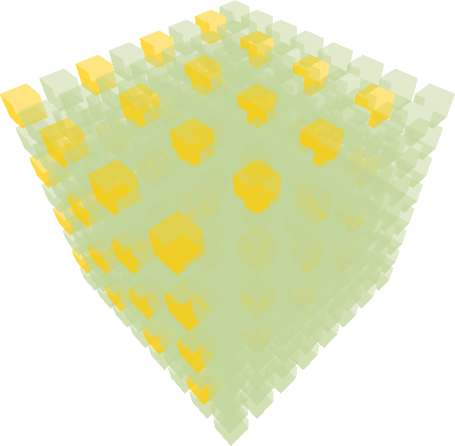
\includegraphics[width=0.3\linewidth]{fig/mixedband3d1.png}
	}	
	\subfloat[]
	{  
		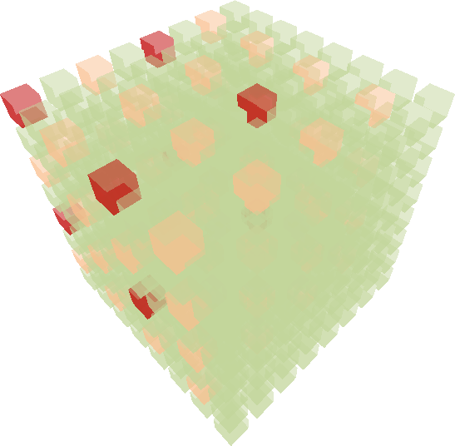
\includegraphics[width=0.3\linewidth]{fig/mixedband3d2.png}
	}	
		\subfloat[]
	{  
		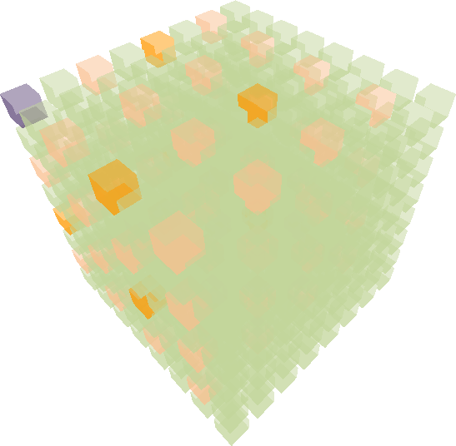
\includegraphics[width=0.3\linewidth]{fig/mixedband3d3.png}
	}	\\
\caption{TODO}
\label{fig:}
\end{figure}

\subsection{Image Denoising with filtering}
\subsection{Image Denoising with DWT and thresholding}
\subsection{Image Denoising with GPU and NVIDIA CUDA}